%% Requires compilation with XeLaTeX or LuaLaTeX
\documentclass[10pt,xcolor={table,dvipsnames},t]{beamer}
\usetheme{UCBerkeley}

\title[Your Short Title]{Interfaces}

\author{Keith Lancaster, Ph.D.}
\institute{Department of Computer Science and Engineering}
\date{}

\begin{document}

\begin{frame}
  \titlepage
\end{frame}

% Uncomment these lines for an automatically generated outline.
%\begin{frame}{Outline}
%  \tableofcontents
%\end{frame}

\section{}

\begin{frame}[c]{Interfaces}
\large
We all deal with interfaces every day - 
\begin{itemize}
	\item We work with user interfaces in software
	\large
	\begin{itemize}
	    \item We create documents in Word, we browse the web using a mouse and keyboard, all without having to know \textit{how} the underlying code works
    \end{itemize}   
    \item We deal people that provide services, where we only need ask for something to be done. We don't need to know \textit{how} the work is accomplished.

\end{itemize}
\end{frame}

\begin{frame}[c]{Interfaces at the Coding Level}
\large
\begin{itemize}

\item The idea behind \textit{encapsulation} is that classes expose an \textit{interface}
through their public methods that allows other classes to use them, \textit{without}
knowing anything about how the functionality is implemented.

\item Operating systems expose \textit{application programmer interfaces} - functions that we call to perform all sorts of operations. We don't (and can't in most cases) know anything about what is going on underneath. 

\item The interface provides a \textit{contract} in a sense. If I call your function, you are telling me to trust that you will complete my request.
\end{itemize}
\end{frame}

\begin{frame}[c]{Interfaces in C++}
\large
\begin{itemize}
	\item Some languages such as Java and C\# have an interface type
	\item Interfaces in these languages have no implementations or state
	\item In C++, an \textit{interface} is an abstract class.
    \begin{itemize}
	    \item So what is the difference between interfaces and abstract classes if they
	are the same in C++? If you fancy a fight, ask on Stack Overflow.
    \end{itemize}
\end{itemize}
\end{frame}

\begin{frame}[c]{Interfaces vs Abstract Classes}
\large
Leaving C++ aside for a moment,
\begin{itemize}
	\item Interfaces provide a view to the outside world of the \textit{behaviour} 
	that you can expect a class to implement
	\item In Java, for example, the naming convention for interfaces is to use "...able" in the name: \texttt{IRunnable},\texttt{IDisposable}, etc.
	\item Java does not have multiple inheritance, so this is a way to provide
	common capabilities across classes where there is already an inheritance
	hierarchy
	\item Some common Java interfaces:\\ \url{http://blog.amitinside.com/Java-_able-Interfaces/}
\end{itemize}

\end{frame}

\begin{frame}[c]{So Again, What is the Diff?}
\large
\begin{itemize}
	\item None, really, at some level
	\item Interfaces are abstract classes. But...an interface by definition
	is there only to specify the behaviour of the class to the outside world. Not
	to provide an implementation or maintain state (i.e., no attributes)
	\item In general, an interface should consist of ONLY pure virtual functions
	\begin{itemize}
	\item As with many things in programming, this is a \textit{guideline}, not
	an absolute rule.
\end{itemize}

\end{itemize}

\end{frame}

\begin{frame}[c]{Example: Mammal Hierarchy}
What do these have in common? What do they \textit{not} have in common?
\center
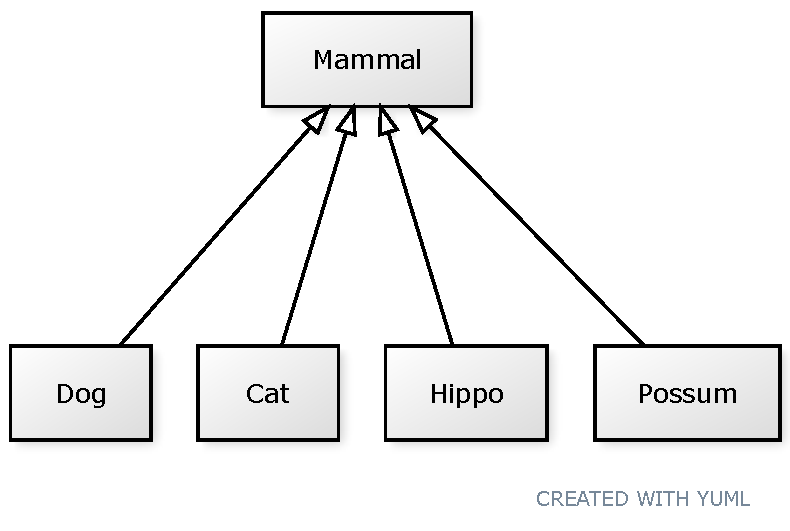
\includegraphics[width=0.6\textwidth]{animal-hierarchy.pdf}
\end{frame}

\begin{frame}[c]{Example: Mammal Hierarchy}
Behaviours that are not common to all in a hierarchy go in 
an interface. We still need the \texttt{Mammal} abstract class
to capture common traits and behaviour across the entire hierarchy
\center 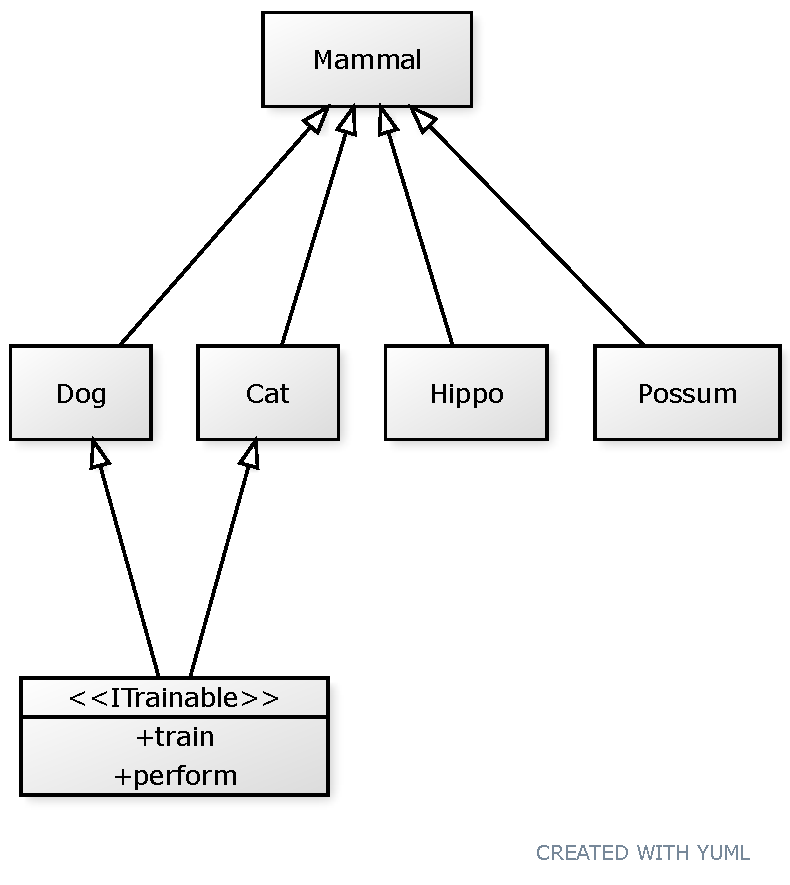
\includegraphics[width=0.4\textwidth]{perform.pdf}
\end{frame}
\begin{frame}[c]{Some Ambiguous Cases}
What say you? Is this the way?
\begin{itemize}
	\item Is \texttt{Vehicle} a base class or an interface?
	\item More generally, should interfaces be nouns?
\end{itemize}
\vspace{0.2cm}
The answer is not always clear. One way of thinking would be to use
an abstract base class when you can say "is a" and an interface when you say
"is".

A cat \textit{is} pettable. You cannot say a cat "is a" pettable.\\
\textbf{Remember:} In C++, this is mostly semantic. An interface \textit{is} an abstract base class.


\end{frame}
\end{document}
